\documentclass[class=NCU_thesis, crop=false]{standalone}

\begin{document}
\chapter{實驗架設與結果討論}

\section{光源製備}

\subsection{雷射光}
雷射光源為 Toptica 的半導體雷射,可產生波長 795 nm 的窄頻雷射

\subsection{單光子}
\label{subsection:single_photon}
雙光子的產生機制為 SPDC,入射一道波長 397.5 nm 的藍光雷射進入 PPKTP 晶體,產生 Type-II 的時間 - 能量糾纏光子對 (time-energy entangled biphoton),波長為 795 nm。
實驗上會將產生出來的雙光子對經過 PBS,將訊號分為 signal 和 idler,以 idler 做為觸發訊號,使 signal 經過 $^{87}Rb$ 原子氣體管與 EOM,讓光子被吸收或對其進行相位的調製,並做 $G^{2}(\tau)$ 的測量,$G^{2}(\tau)$ 的定義如 (\ref{eq:g2_definition})。

\begin{equation}
    G^{2}(\tau)=\frac{4\Gamma_{s}\Gamma_{i}}{\Gamma_{s}+\Gamma_{i}}\left\{\begin{matrix}
        e^{\Gamma_{s}\tau} & ,\tau<0\\
        e^{-\Gamma_{i}\tau} & ,\tau>0
        \end{matrix}\right.
\label{eq:g2_definition}
\end{equation}

此為二階強度關聯函數 (second-order intenstiy correlation function),$\tau$ 為兩顆單光子抵達探測器的時間差。在符合準相位匹配條件 (quasi phase matching condition) 時能最有效率的產生雙光子,實際測量結果如\cref{fig:single_photon_g2},此光子之時間波包寬度約為 100 ns,頻寬為 4.5 MHz。

\fig[0.5][fig:single_photon_g2][!htb]{temp.png}[糾纏光子對之 $G^{2}(\tau)$ 量測]

為了找到符合準項未匹配條件的入射光波長與晶體溫度,實驗上我們先將入射光的頻率固定在 105489 MHz,改變晶體溫度測量雙光子的產生率 (biphton rate),結果如\cref{fig:temp_scan_g2}黑線,在 39.91$^{\circ}C$ 至 40.10$^{\circ}C$ 有四組符合條件的模態,若讓其中一顆光子經過 $^{87}Rb$ 原子氣體管,並做相同的量測,結果如\cref{fig:temp_scan_g2}紅線,可以發現第二和第三個的模態雖有明顯的吸收,但吸收率不高,我們認為這是因為晶體所產生的光子為多模 (multi-mode) 而非單模 (single-mode),同時產生了兩種以上頻率的單光子,儘管其中一個頻率的光子能完全被吸收,其他頻率的光子仍會透射,因此無法讓透射率趨近於零。為了確認這想法,我們在探測器前面加上一個頻寬為 60 MHz 的 Etalon 濾波器,只允許特定頻率附近的光通過,並在沒放 $^{87}Rb$ 原子氣體管時改變晶體溫度,重新測量產生率,有無 Etalon 濾波器測量之結果比較如\cref{fig:temp_scan_g2_with_etalon},黑色為沒放 Etalon 濾波器時測量到的訊號,紅色經過濾波後之訊號,兩者相比可明顯看出,有放濾波器時能將其他產生效率較低的模態過濾掉,一次只讓一個特定頻率區間內的光通過。此時再將 $^{87}Rb$ 原子氣體管放回,並對其中第二和第三個模態進行相同的量測,結果如\cref{fig:absorption_etalon_temp_scanning},黑線為加上 Etalon 過濾之後測到的訊號,若放上 $^{87}Rb$ 原子氣體管讓光子通過,測量結果如藍線,光子幾乎完全被吸收,與\cref{fig:temp_scan_g2}相比,可明顯看出,在過濾前的光源的確有其他頻率的成分,要避免其他頻率成分影響後續的實驗與分析,需加上 Etalon 濾波器。

\fig[0.75][fig:temp_scan_g2][!htb]{temp_scanning.png}[調整溫度測量雙光子產生率,黑線為直接對雙光子進行量測;紅線為先讓其中一顆單光子通過 $^{87}Rb$ 氣體管再測量,其中第二和第三個模態有部分吸收。][調整溫度測量雙光子產生率]

\fig[0.75][fig:temp_scan_g2_with_etalon][!htb]{temp_scanning_with_etalon.png}[黑色為無濾波器時測量之訊號,在二與三個模態附近測量到一些明顯的訊號,表示我們的單光子非單模;紅線為經過濾波器測量到的訊號,此時就只允許特定頻率透射。][調整溫度測量雙光子產生率(加上濾波器)]

\begin{figure}[!hbt]
    %\captionsetup[subfigure]{labelformat=empty} % 完全隱藏圖號
    \centering
    \subcaptionbox
        {第二個模態
        \label{fig:subfig_fig1}}
        {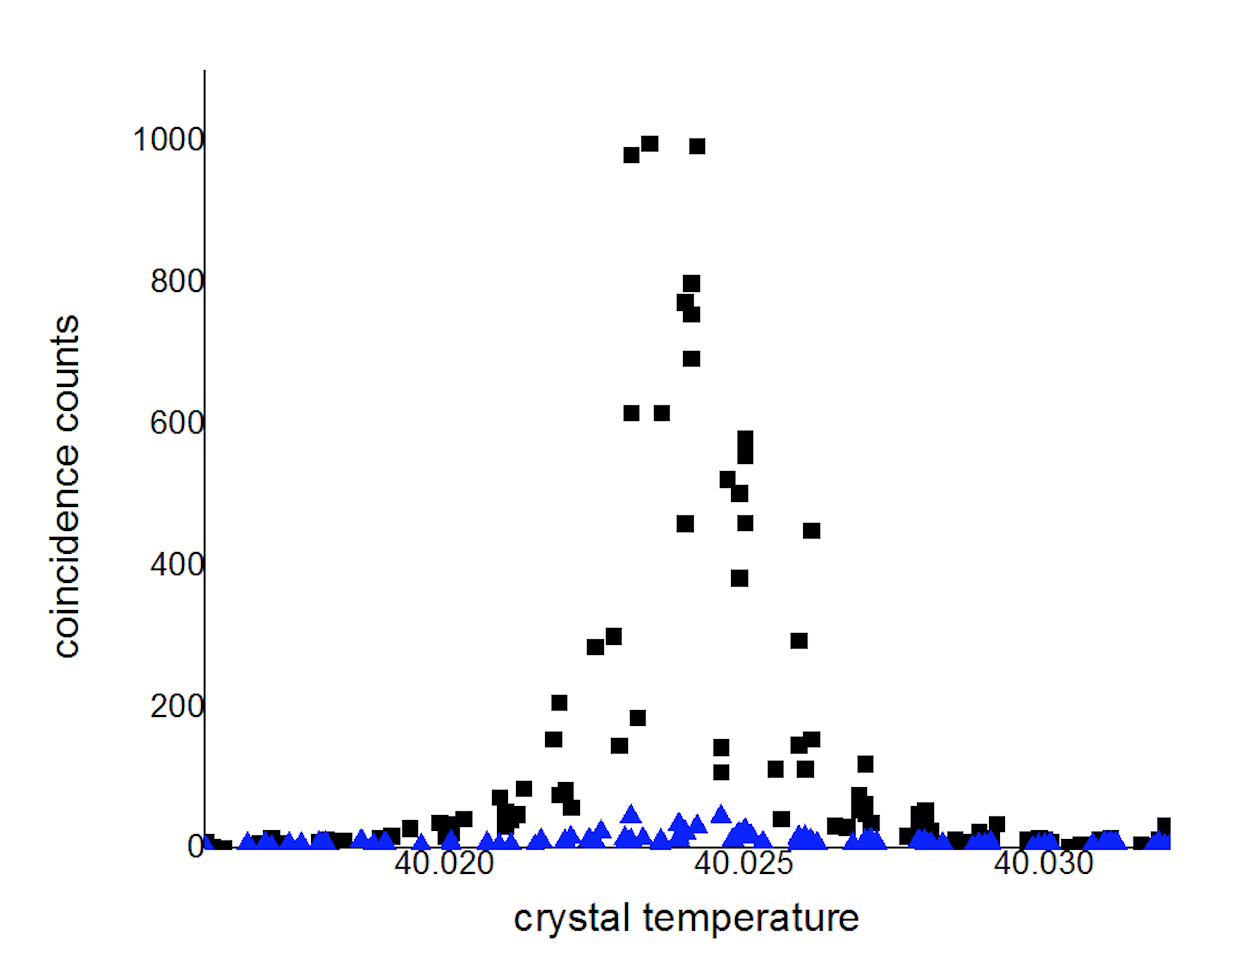
\includegraphics[width=0.4\linewidth]{second_mode_absorption.png}}
    ~~~~
    \subcaptionbox
        {第三個模態
        \label{fig:subfig_fig2}}
        {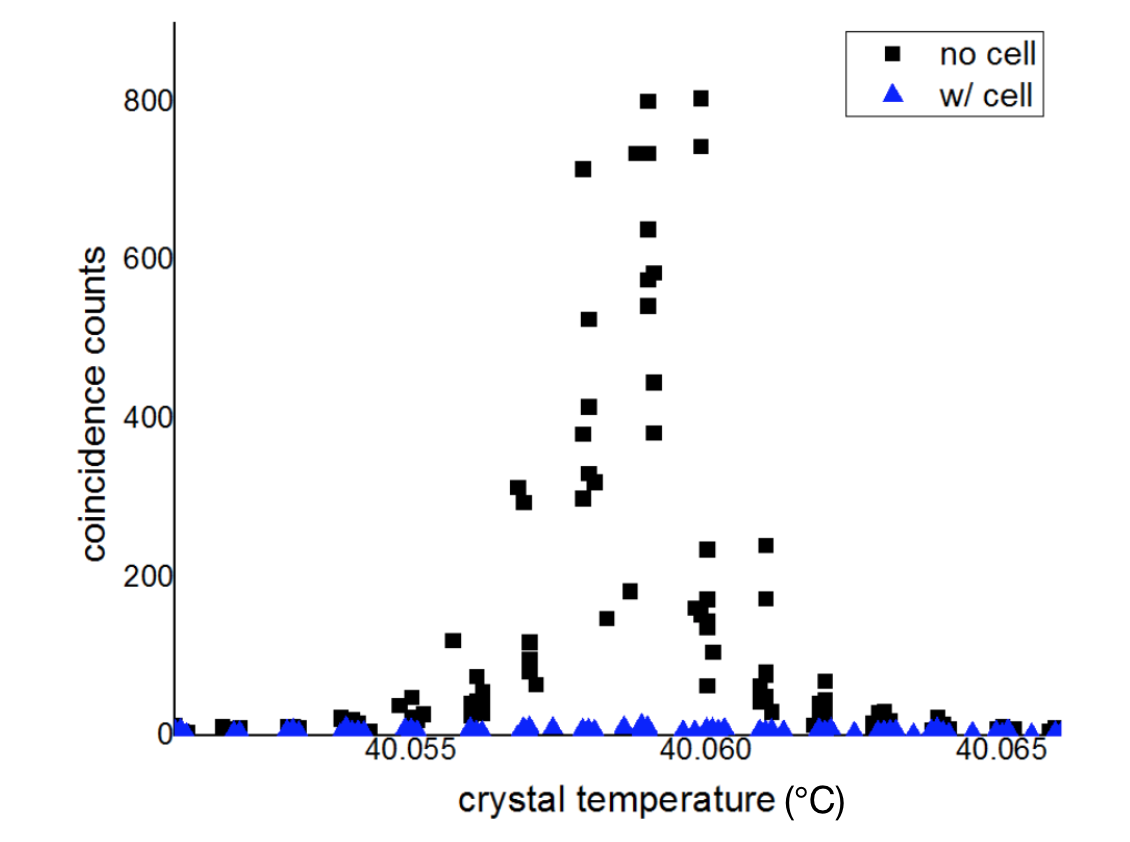
\includegraphics[width=0.4\linewidth]{third_mode_absorption.png}}
    \caption{經過 Etalon 濾波後光子之吸收}
    \label{fig:absorption_etalon_temp_scanning}
\end{figure}

\section{雷射頻譜量測}

實驗光路架設如\cref{fig:laser_spectrum_setup},我們將窄頻雷射通過兩台 EOM 對其進行相位調製,第一台為展頻用,第二台用來做反向的調製還原頻譜,再以 Fabrty-Perot 干涉儀去測量頻譜。

\fig[0.5][fig:laser_spectrum_setup][!htb]{temp.png}[雷射頻譜量測光路圖]

在兩台 EOM 都關閉的情況下,可以測到波長 795 nm 雷射的頻譜,結果如圖,以此 Fabry-Perot 的解析度掃出的雷射頻寬約為 60 MHz。

\fig[0.75][fig:label][!htb]{compress_comparison.png}[以頻寬 60MHz 的 Fabry-Perot 干涉儀掃出之雷射頻譜][雷射頻譜]

若只開啟第一台 EOM,在 10 Gb/s 隨機訊號的調製下可將窄頻雷射光的頻譜展至 10 GHz 寬,但由於我們的使用的 Fabry-Perot FSR 僅 10 GHz,無法涵蓋完整的頻率區間,會使測量的結果失真,要想掃出完整展開的頻譜需使用 FSR 20 GHz 以上的干涉儀,所以下面會先以 2 Gb/s 的訊號來測試展頻的結果是否符合理論模擬。

\subsection{2 Gb/s 隨機訊號之相位調製}
先以 2 Gb/s 隨機訊號進行相位調製,只開啟第一台能將頻譜展至 $\pm$5 GHz 寬,如下圖。

\fig[0.75][fig:label][!htb]{2_31_spread_2GHz.png}[2 Gb/s 訊號之展頻頻譜]

頻譜的形狀大致上與理論相符,但在 $\pm$2 GHz 的位置有一個突起的訊號,這是由於隨機訊號的上升與下降時間不夠快所致,若在數值模擬中把隨機訊號加上約 30 ps 的上升與下降時間(如圖),則會出現類似的結果,如圖:

\begin{figure}[!hbt]
    %\captionsetup[subfigure]{labelformat=empty} % 完全隱藏圖號
    \centering
    \subcaptionbox
        {caption\_2
        \label{fig:subfig_fig1}}
        {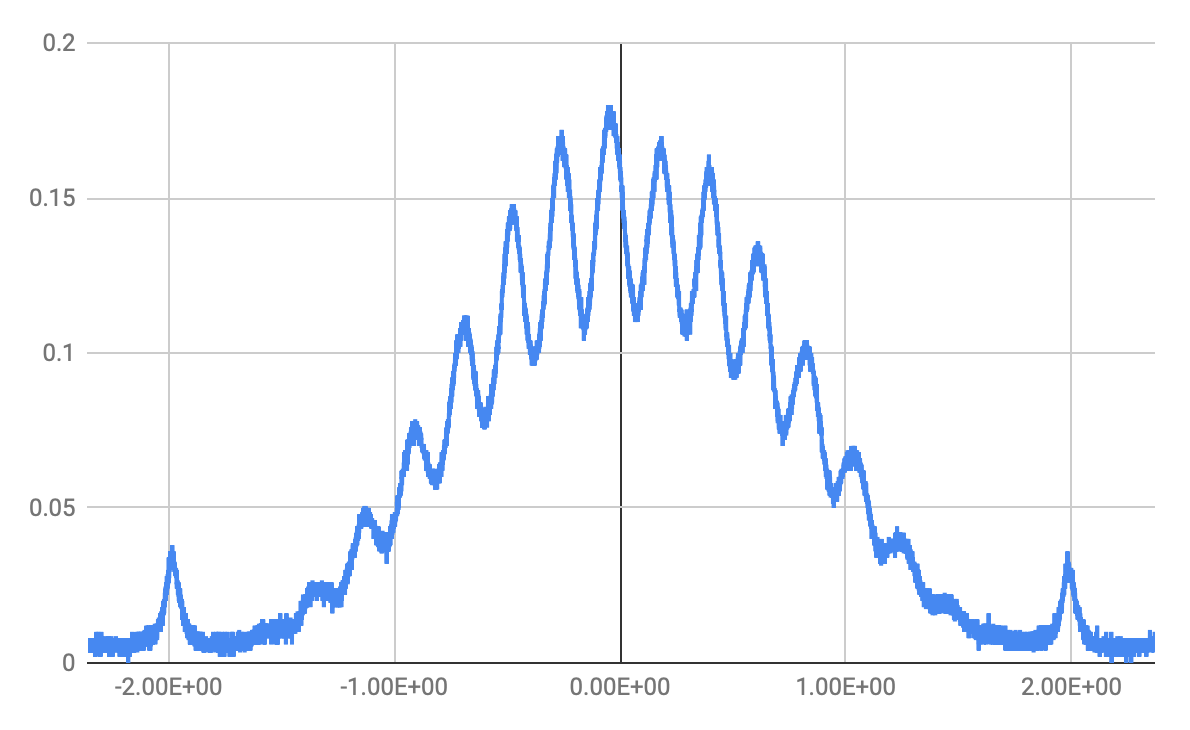
\includegraphics[width=0.4\linewidth]{2_7_spread_2GHz.png}}
    ~~~~
    \subcaptionbox
        {caption\_2
        \label{fig:subfig_fig2}}
        {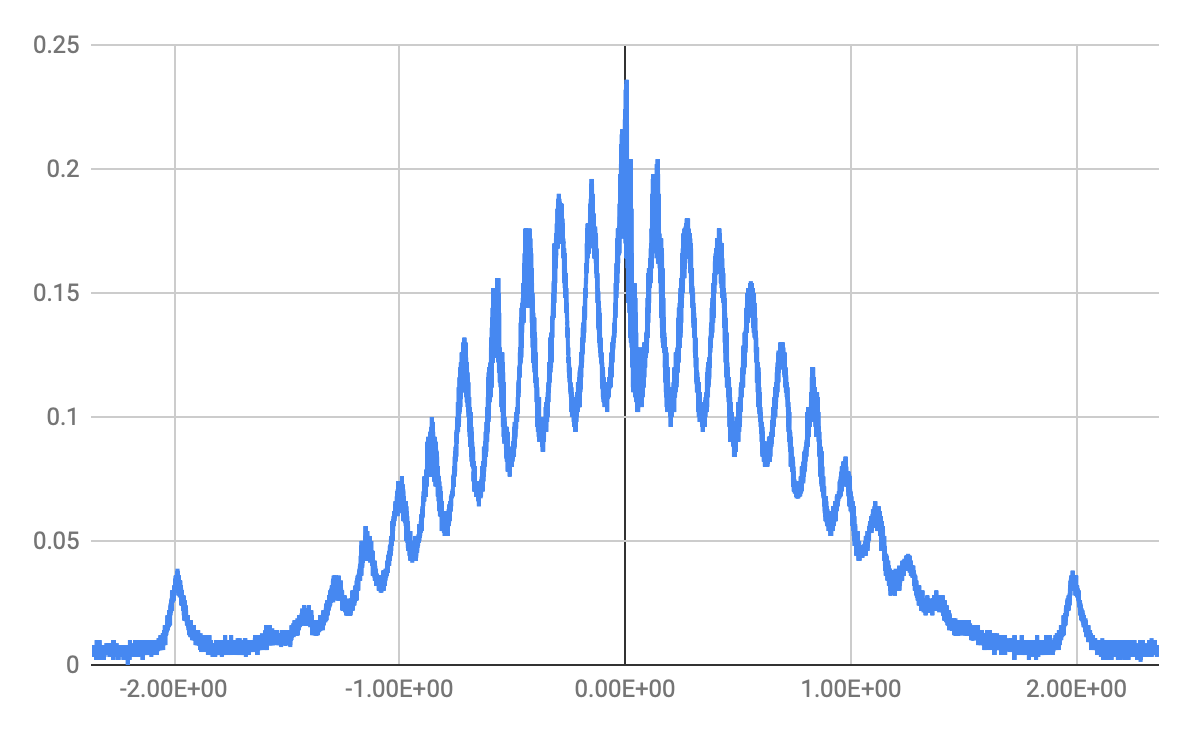
\includegraphics[width=0.4\linewidth]{2_15_spread_2GHz.png}}
\end{figure}

% \fig[0.5][fig:label][!htb]{temp.png}[修正前後之隨機訊號]
% \fig[0.5][fig:label][!htb]{temp.png}[修正後展頻頻譜]

此外,還可隱約看出該頻譜的包絡線有週期振盪的訊號,原因為我們使用的隨機訊號實際上是個重複出現的週期訊號,每個週期有 $2^{31}-1$ 個位元,若把位元數調為 $2^{15}-1$ 或者 $2^{7}-1$ 則可看到週期更大的震盪訊號,測量結果如\cref{fig:different_length_PRBS}。

\begin{figure}[!hbt]
    %\captionsetup[subfigure]{labelformat=empty} % 完全隱藏圖號
    \centering
    \subcaptionbox
        {週期 $2^{15}-1$ 位元之偽隨機訊號
        \label{fig:subfig_fig1}}
        {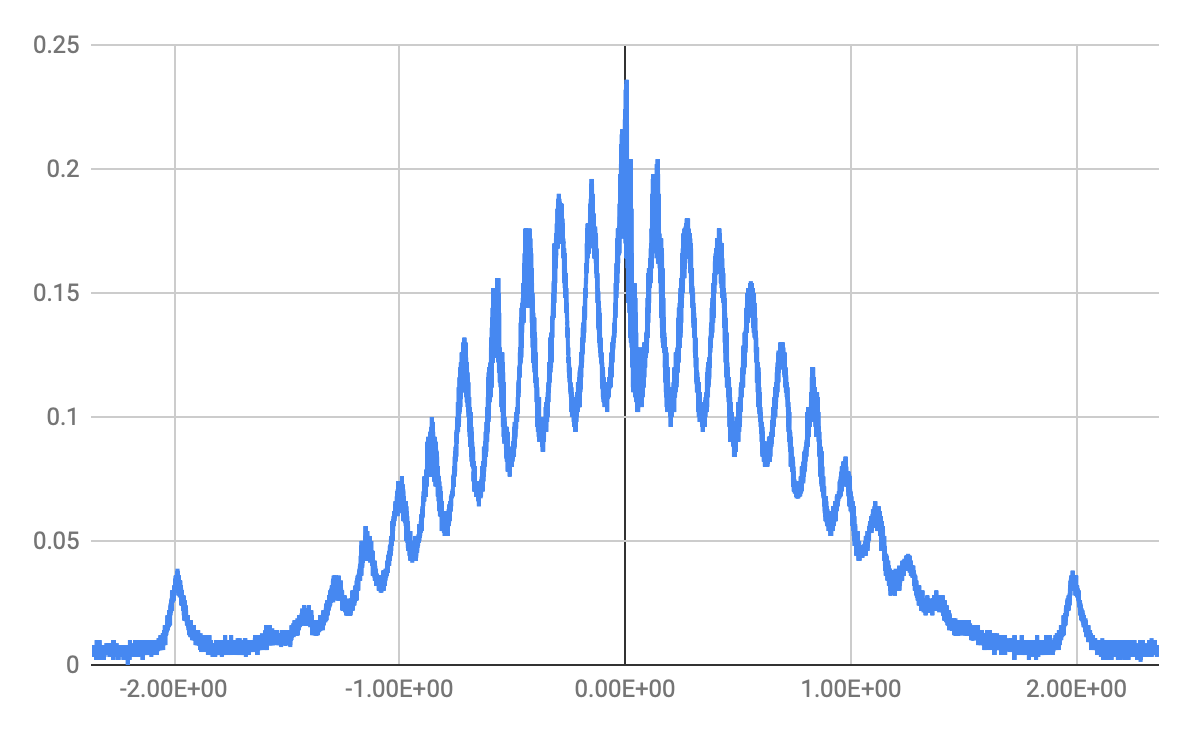
\includegraphics[width=0.4\linewidth]{2_15_spread_2GHz.png}}
    ~~~~
    \subcaptionbox
        {週期 $2^{7}-1$ 位元之偽隨機訊號
        \label{fig:subfig_fig2}}
        {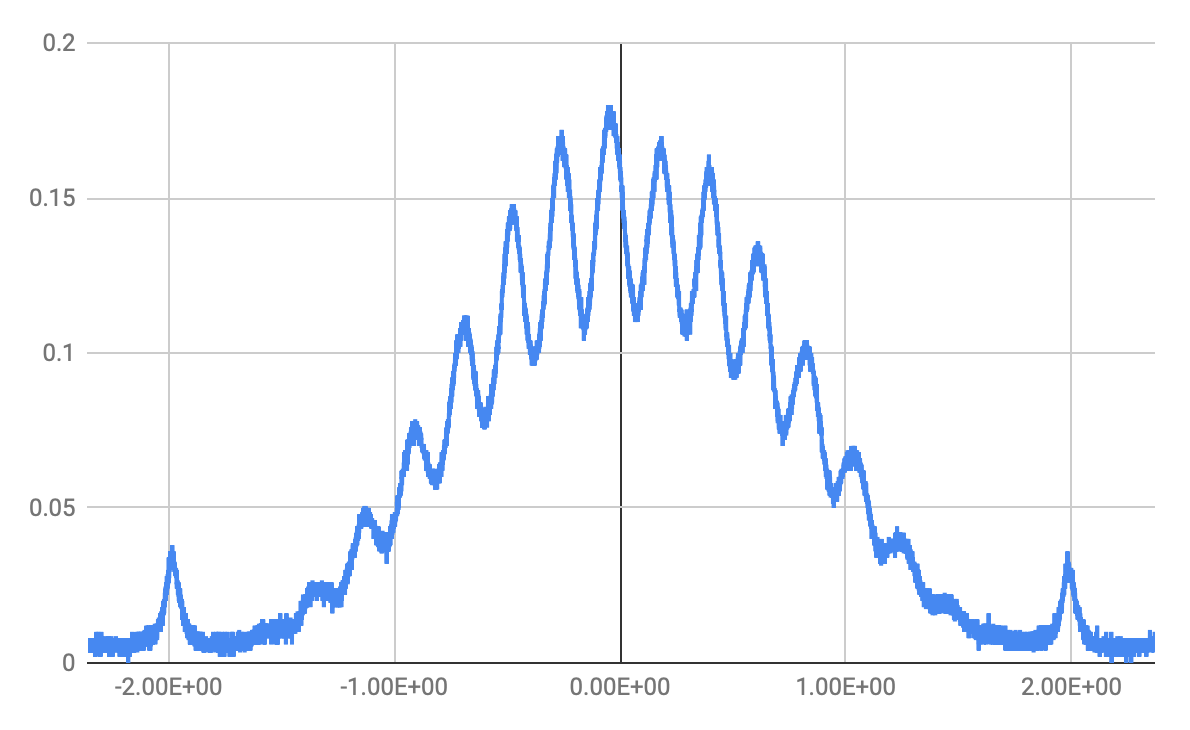
\includegraphics[width=0.4\linewidth]{2_7_spread_2GHz.png}}
    \caption{偽隨機訊號週期與展頻頻譜震盪之關係}
    \label{fig:different_length_PRBS}
\end{figure}

從以上測量的頻譜可以看出,調製後的頻寬與理論計算的結果一致,所以我們認為 10 Gb/s 的隨機訊號能將訊號展至 $\pm$10 GHz 寬。

\subsection{10 Gb/s 隨機訊號之相位調製}

當兩台 EOM 同時開啟時,理論上要能將展寬的頻譜還原成調製前的狀態,但從\cref{fig:10gbs_compress_sprectrum} 的實驗結果可以看出,壓縮回來的頻譜與調製前相比,中心頻率的強度僅為本來的 80\%,若將電壓放大來看(如\cref{fig:compress_amplified_compare})可以觀察到,在調製前所有能量皆集中於中心頻率附近,但經過兩台 EOM 調製後,仍有部分能量分散在其他頻率沒被還原,導致中心頻率的強度降低。造成頻譜還原效果不佳的可能原因為,兩個隨機訊號的形狀與穩定度皆不同(如\cref{fig:amplified_signal}),導致無法將相位做反向的調製,使訊號完美還原成最初的狀態。

\fig[0.5][fig:10gbs_compress_sprectrum][!htb]{compress_comparison_100.png}[10 Gb/s 訊號壓縮後頻譜]

\fig[0.5][fig:compress_amplified_compare][!htb]{compress_zoom_in.png}[放大後之電訊號,紅線為未經調製的雷射頻譜,黑線為兩次調製後的訊號,雖能大致上將頻寬從 10 GHz 壓回 60 MHz,但從圖中可發現,中心以外的頻率仍能測到一些訊號。][初始頻譜與壓縮頻譜放大比較圖]

\begin{figure}[!hbt]
    %\captionsetup[subfigure]{labelformat=empty} % 完全隱藏圖號
    \centering
    \subcaptionbox
        {第一台 EOM 
        \label{fig:subfig_fig1}}
        {\includegraphics[width=0.4\linewidth]{amp_data.bmp}}
    ~~~~
    \subcaptionbox
        {第二台 EOM
        \label{fig:subfig_fig2}}
        {\includegraphics[width=0.4\linewidth]{amp_data_bar.bmp}}
    \caption{經過放大器,進入 EOM 用以調製的兩組隨機訊號眼圖}
    \label{fig:amplified_signal}
\end{figure}

\section{$^{87}Rb$ 經相位調製後的原子吸收譜}

如章節 \ref{section:simulation_absorption} 所提,當光子的頻率很接近原子的躍遷能階時,光會被吸收,實驗上可以\cref{fig:laser_spectrum_setup}的架設,將 Farby-Perot 干涉儀換成光二極體 (photodiode) 收光,連續調變入射光的頻率,測量透射 $^{87}Rb$ 原子氣體管的光強,從\cref{fig:abs_spec} 藍線可以觀察到,在特定的兩個頻率位置附近光會被原子吸收,穿透率特別低。本實驗主要的目的為透過展頻技術,降低光子與原子的交互作用,使光子能不被吸收而增加透射率,所以若將第一台 EOM 開啟,將雷射的頻寬從 60 MHz 展至 10 GHz,此時的吸收譜如\cref{fig:abs_spec} 紅線,在經過展頻後,無論在哪個頻率下光皆能大部分透射原子,調製前的光在 105 GHz 與 112 GHz 會被完全吸收,調製後卻有 75\% 的光能透射原子,就如隱形了一般,展頻能降低光子受環境的影響。

\fig[0.75][fig:abs_spec][!htb]{absorption_spectrum_spread.png}[調製後的如原子吸收譜,黑線為沒放 $^{87}Rb$ 原子氣體管時的訊號;藍線為調製前 $^{87}Rb$ 原子氣體管的吸收譜;紅線為展頻後的吸收譜。][調製後的銣原子吸收譜]
\todo[inline]{重畫,調整座標軸}

\section{單光子相位調製對原子吸收之影響}
從前一小節的實驗結果能得知,$^{87}Rb$ 的躍遷頻率約在 105 GHz 與 112 GHz 附近,這時我們將光源從窄頻雷射換成單光子,並透過改變入射光的頻率與晶體溫度,將單光子的頻率調至 112300 MHz,使其能被原子吸收,再以\cref{fig:single_photon_no_etalon} 的光路架設,對光子進行相位調製與測量。

\fig[0.5][fig:single_photon_no_etalon][!htb]{temp.png}[單光子量測光路圖]

當兩台 EOM 皆關閉時,頻寬約為 4.5 MHz 的單光子會幾乎完全被原子吸收,光無法透射氣體管,但若對其進行 $G^{2}(\tau)$ 測量,卻會測到訊號,如\cref{fig:remaining_mod_g2},原因如章節 \ref{subsection:single_photon} 所述,是由於我們晶體產生的單光子源非單模 (single-mode),其中還存在符合其他組準相位匹配條件 (quasi phase matching condition) 所產生的光,若要去除那些光子對實驗的影響,在此小節的數據處理上,我們直接將其當作雜訊扣除,只保留主要模態的光;下一小節的實驗中,我們會外加一個 Etalon 濾波器,只讓 112300 MHz 附近的光通過。

\fig[0.75][fig:remaining_mod_g2][!htb]{no_etalon_with_cell.png}[單光子通過 $^{87}Rb$ 氣體管之 $G^{2}(\tau)$ 量測,黑線為沒放氣體管時測到的訊號,放了氣體管後,其他模態的光因不在吸收頻率附近而能透射原子團不吸收,所以會測到紅線的訊號。][單光子通過 $^{87}Rb$ 氣體管之 $G^{2}(\tau)$ 量測]

若開啟第一台 EOM,以 10 Gb/s 的隨機訊號對單光子進行相位調製,可以讓單光子的頻寬從 4.5 MHz 展至 10 GHz,使大部分的光可以透射 $^{87}Rb$ 氣體不被吸收,扣除雜訊後的 $G^2(\tau)$ 的測量結果如\cref{fig:spread_absorption_g2},透射率為 76\%。另外,此時若將 $^{87}Rb$ 氣體管移除,直接測量展頻後的訊號,能發現單位時間測量到的光子數與調製前相差不多,比較如\cref{fig:spread_or_not},印證了本章第一小節的結論——相位調製僅改變頻率的分佈,不會影響光強。

\fig[0.7][fig:spread_absorption_g2][!htb]{no_etalon_spread.png}[黑線為沒被放氣體管也沒調製時的 $G^{2}(\tau)$ 量測,紅線為展頻光子被部分吸收後之訊號,可以以兩者 concidence counts(也就是圖下面積)的比值來計算透射率,約為 76\%][展頻單光子被部分吸收後 $G^{2}(\tau)$ 量測]

\begin{figure}[!hbt]
    %\captionsetup[subfigure]{labelformat=empty} % 完全隱藏圖號
    \centering
    \subcaptionbox
        {調製前 
        \label{fig:subfig_fig1}}
        {
\includegraphics[width=0.4\linewidth]{temp.png}}
    ~~~~
    \subcaptionbox
        {調製後
        \label{fig:subfig_fig2}}
        {
\includegraphics[width=0.4\linewidth]{temp.png}}
    \caption{沒通過 $^{87}Rb$ 氣體管之單光子 $G^{2}(\tau)$ 量測。有無相位調製時的雙光子產生率幾乎相同}
    \label{fig:spread_or_not}
\end{figure}

從前述的結果可知,未經調製的窄頻單光子會幾乎被 $^{87}RB$ 原子吸收,無法透射氣體管,透射率幾乎為零,但經過 10 Gb/s 隨機訊號的調製後,可讓透射率提升至 76%,如同穿上隱形斗篷般,能大部分的光子不會與原子產生交互作用,直接穿透原子團。

\section{雷射光相位調製對原子吸收之影響}
在上一小節中,我們對單光子進行相位調製,觀察展頻對吸收率之影響,為確定此現象在不同系統下能維持一致性,我們將\cref{fig:single_photon_no_etalon}光路架設的光源改為雷射光,單光子探測器改用光二極體,並將雷射調至與單光子同樣的波長去進行相同的量測,實驗結果如\cref{fig:laser_no_etalon},與單光子的量測結果相近,調製前的光幾乎會全部被原子團吸收,但經過展頻後的雷射光能有約 80\% 的穿透率,也能達到隱形斗篷的效果。

\fig[0.75][fig:laser_no_etalon][!htb]{laser_no_etalon.png}[雷射光相位調製對穿透率之影響,最上面三條線(藍、紅與黃色)為沒放$^{87}RB$ 原子氣體管時之量測,無論是展頻還是壓縮,相位調製皆不會影響光強;中間兩條線(綠色與橘色)為展頻後通過氣體管所測得的訊號,約 80\% 的光能因相位調製而穿透原子團而不被吸收;最下面的藍線為兩台 EOM 關閉時測到的訊號,未經調製的光會幾乎都被原子吸收。][雷射光相位調製對穿透率之影響]

\section{不同展頻頻寬對吸收率之影響}
由章節 \ref{section:simulation_absorption} 的模擬可知,使用越高頻的隨機訊號去展頻可提升光子隱形的效果,為驗證此理論,我們分別使用 2, 4, 6, 8, 10 Gb/s 的隨機訊號去展頻,並透射原子團測量穿透率,實驗結果如\cref{fig:different_gbs_abs},從結果可看出,無論是雷射光或單光子,頻寬越大,吸收率越低,使用越高的頻率去進行調製,的確能增加光子的隱匿性,降低環境或竊聽者的影響。

\fig[0.75][fig:different_gbs_abs][!htb]{main_result.png}[黑色為數值模擬;紅線與藍線分別為雷射光與單光子的實驗測量結果,數據點的值為數次測量的平均,帶狀的寬度為測量的標準差。單光子的標準差較大是實驗穩定度不佳造成的。][改變展頻頻率對吸收率之影響]

此外,可以看出單光子的透射率皆比雷射光低一些,或許是因為單光子較容易被原子團吸收所致。

\section{單光子頻譜壓縮}

從前兩小節的結果可知,使用展頻技術可以有效的降低環境對光子的影響,但若考量到接收訊息端可能會需要光子原始的相位資訊,或者需要讓光子與 $^{87}Rb$ 原子進行交互作用,我們必須要開啟第二台 EOM 進行反向的調製,盡量使光子還原到原先的狀態,若以\cref{fig:single_photon_no_etalon}的光路架設,除了第一台 EOM 外,將第二台也開啟,由於相位調製不影響光強與波形,單就 $G^{2}(\tau)$ 的測量無法得知頻譜的變化,因此要將光路架設改為\cref{fig:single_photon_with_etalon},在單光子探測器前加上 Etalon 濾波器,限制只讓頻寬 60 MHz 內的光通過,如此一來,只要能測到訊號就代表部分光子的頻寬有被壓窄至 60 MHz 內,另一方面,這也可以將上一小節及提的雜訊去除。

\fig[0.75][fig:single_photon_with_etalon][!htb]{temp.png}[加上濾波器之單光子量測光路圖]

以\cref{fig:single_photon_with_etalon}的光路架設,只開啟第一台 EOM 時,被展頻的單光子能大部分透射原子團,但由於 Etalon 的過濾,頻寬 10 GHz 的光子幾乎無法抵達探測器,因而測不到明顯的訊號,結果如\cref{fig:spread_single_photon_with_etalon}。若將第二台 EOM 也開啟,將已展頻且被部分吸收的單光子頻譜壓縮,則能再次測到訊號,如\cref{fig:compress_single_photon_with_etalon},與調製前且沒放氣體管時的初始訊號相比,透射率為 42.3\%。

\begin{figure}[!hbt]
    %\captionsetup[subfigure]{labelformat=empty} % 完全隱藏圖號
    \centering
    \subcaptionbox
        {只開啟第一台 EOM,將展頻單光子通過原子團,雖然能大部分透射不被吸收,但由於光子的頻寬 10 GHz,遠小於 Etalon 濾波器的 60 MHz,所以測不到訊號。
        \label{fig:spread_single_photon_with_etalon}}
        {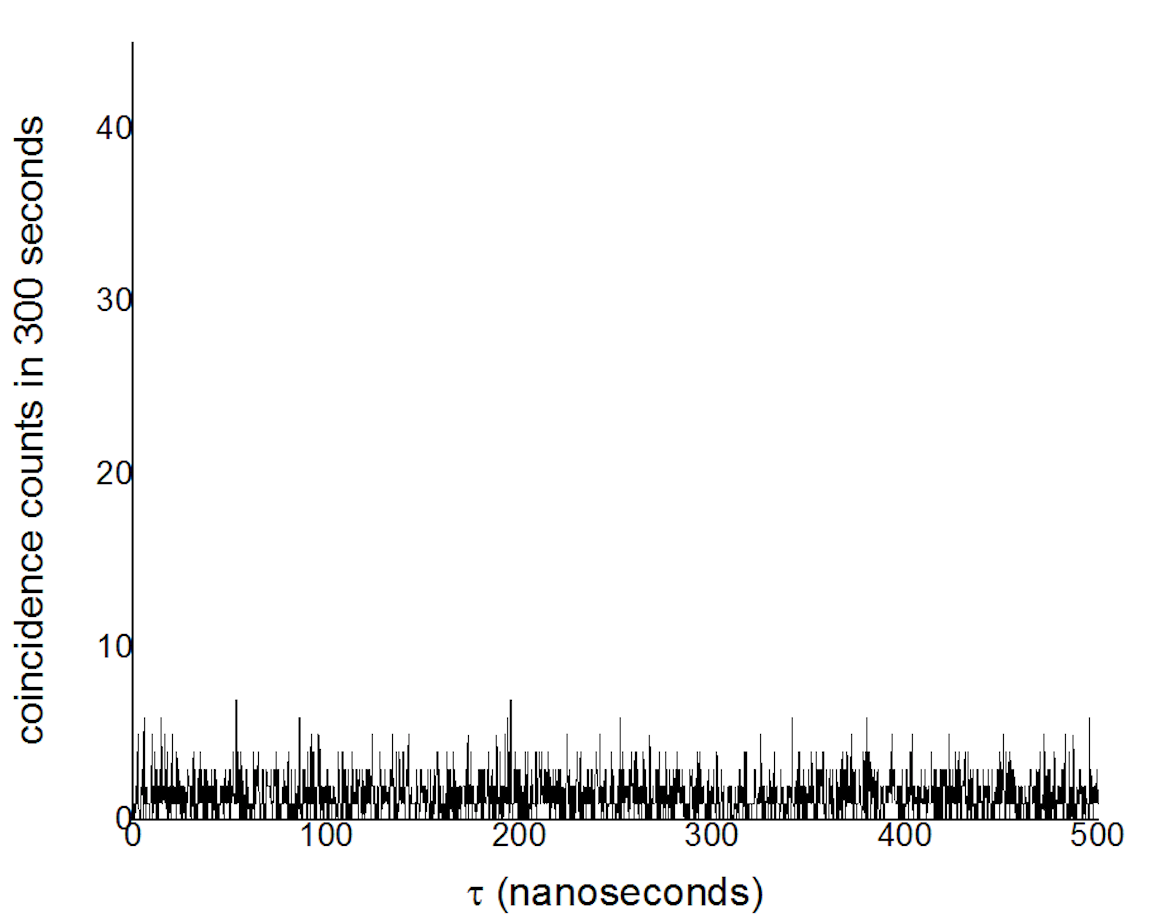
\includegraphics[width=0.4\linewidth]{heat_cell_spread_with_etalon.png}}
    ~~~~
    \subcaptionbox
        {兩台 EOM 同時開啟,將已展頻的單光子頻譜壓縮,使光子再次現形,能透射 Etalon 濾波器,被探測器偵測到。
        \label{fig:compress_single_photon_with_etalon}}
        {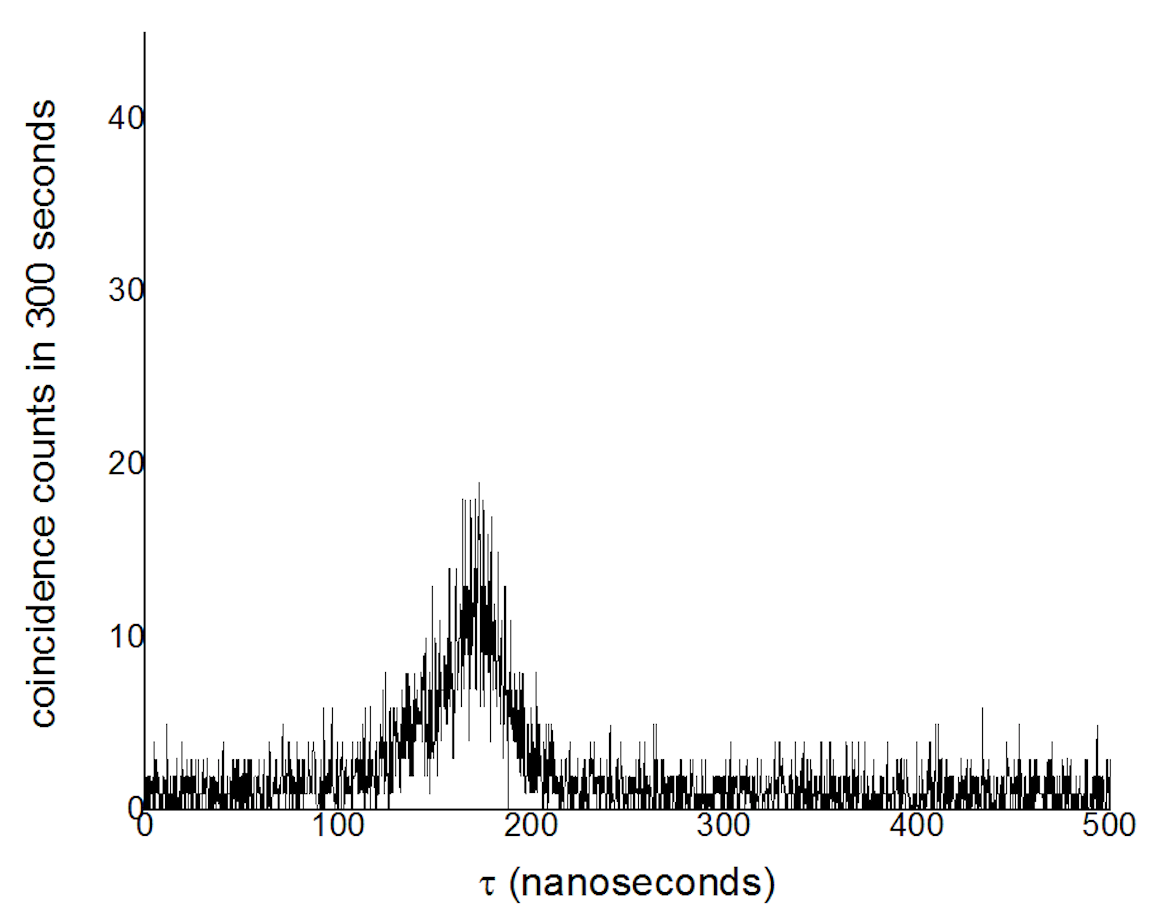
\includegraphics[width=0.4\linewidth]{heat_cell_compress_with_etalon.png}}
    \caption{加上 Etalon 濾波器之單光子 $G^{2}(\tau)$ 量測}
    \label{fig:single_photon_with_etalon}
\end{figure}

為了知道原子吸收對於單光子頻譜的壓縮有何影響,我們以同樣的光路架設,在沒放 Etalon 濾波器時,同時開啟兩台 EOM,測量結果如\cref{fig:nocell_compress_with_etalon}黑線,與調製前的訊號相比,透射率為 77.9\%;放上 $^{87}Rb$ 原子氣體管後的訊號為紅線,透射率為 42.3\%。

\fig[0.75][fig:nocell_compress_with_etalon][!htb]{no_cell_compress_with_etalon.png}[在兩台 EOM 同時開啟時測量 $G^{2}(\tau)$,黑線為沒經過 $^{87}Rb$ 原子氣體管時之量測;紅線為透射 $^{87}Rb$ 原子氣體管之訊號。][原子吸收對單光子壓縮比較圖]

\section{雷射光頻譜壓縮}

同樣的,我們以上一小節相同的架設,將光源換成雷射光,單光子探測器改為光二極體,且進行同樣的測量,結果如\cref{fig:no_cell_compress_laser},與單光子的量測結果相近,經展頻後在壓縮的光,約 70\% 能通過 Etalon 濾波器,若在中間放氣體管使部分光被吸收,僅 40\% 的光能通過 Etalon,被重新壓回窄頻雷射

\fig[0.75][fig:no_cell_compress_laser][!htb]{laser_modulation_with_etalon.png}[原子吸收對雷射光壓縮品質比較圖]
\todo[inline]{補上另一條紅色的線}

\section{誤差分析與模擬修正}

由相位調製的基本原理可知,若輸入兩台 EOM 的隨機訊號符合式 () 的條件,則能完美的將光的相位與頻譜還原成最初的狀態,在我們實驗中所使用的窄頻雷射與單光子,頻寬皆遠小於 Etalon 濾波器的頻寬,在沒原子團吸收的狀況下,被展頻再壓縮的光應該要能 100\% 通過 Etalon,這與實驗測量的結果不符,我認為主要的可能原因為隨機訊號的品質不佳所致,兩個訊號從 PRBS 輸出時的波形如\cref{fig:prbs_eye},兩者形狀不一致,且上下不對稱,若在經過延長線與高頻訊號放大器波形則變為\cref{fig:amp_prbs_eye},兩者變得更不一致,有著不一樣的波形、穩定度、上升時間、下降時間與交叉位置 (crossing),這些因素都會使兩台 EOM 的調製無法互相抵消,讓相位無法還原至最初的狀態。除此之外,也有能是因為兩台 EOM 對高頻訊號的響應不同,也會影響調製的結果。

\begin{figure}[!hbt]
    %\captionsetup[subfigure]{labelformat=empty} % 完全隱藏圖號
    \centering
    \subcaptionbox
        {第一台 EOM
        \label{fig:subfig_fig1}}
        {\includegraphics[width=0.4\linewidth]{data.bmp}}
    ~~~~
    \subcaptionbox
        {第二台 EOM
        \label{fig:subfig_fig2}}
        {\includegraphics[width=0.4\linewidth]{data_bar.bmp}}
    \caption{PRBS 輸出之訊號眼圖(放大前)}
    \label{fig:prbs_eye}
\end{figure}

\begin{figure}[!hbt]
    %\captionsetup[subfigure]{labelformat=empty} % 完全隱藏圖號
    \centering
    \subcaptionbox
        {第一台 EOM
        \label{fig:subfig_fig1}}
        {\includegraphics[width=0.4\linewidth]{amp_data.bmp}}
    ~~~~
    \subcaptionbox
        {第二台 EOM
        \label{fig:subfig_fig2}}
        {\includegraphics[width=0.4\linewidth]{amp_data_bar.bmp}}
    \caption{PRBS 輸出之訊號眼圖(放大後)}
    \label{fig:amp_prbs_eye}
\end{figure}

為了確認上述的因素所造成的影響,根據\cref{fig:amp_prbs_eye}的測量結果,修正模擬時使用的隨機訊號,修正的參數如 \cref{tab:paras},並將實驗結果與理論模擬整理成 \cref{tab:spread_abs}



\begin{table}[h]
    \centering
    \caption{數值模擬參數修正}
    \begin{tabular}{| c | c | c | c |}
\hline
         & jitter & amplitidu & rising \& falling
    \\ \hline
    \ce{EOM 1} & 14 ps & $\pm$7.7\% & 38 ps\\ \hline
    \ce{EOM 2} & 16 ps & $\pm$16.7\% & 144 ps\\ \hline
    \end{tabular}
    \label{tab:paras}
\end{table}

\begin{table}[h]
    \centering
    \caption{展頻後的光經過 $^{87}Rb$之穿透率}
    \begin{tabular}{| c | c | c | c | c |}
\hline
         & 修正前理論 & 修正後理論 & 雷射光實驗 & 單光實驗
    \\ \hline
    穿透率 & 79.1\% & 73.8\% & 76.0\% & 79.6\%\\ \hline
    \end{tabular}
    \label{tab:spread_abs}
\end{table}

\end{document}